\documentclass{article}
\usepackage[utf8]{inputenc}
\usepackage[margin=1in]{geometry}
\usepackage{tikz}
\usepackage{tikz-qtree}

\title{Data Structures: Problem Set 3}
\author{Jackie Luo}
\date{April 2, 2015}

\begin{document}
\maketitle

\section{Theory}

\subsection{}

\begin{figure}[ht]
\centering
\begin{tikzpicture}
\Tree [.2 ]
\end{tikzpicture}
\caption{Tree is balanced, no rotation required}
\end{figure}

\begin{figure}[ht]
\centering
\begin{tikzpicture}
\Tree [.2 1 \edge[draw=none]; {} ]
\end{tikzpicture}
\caption{Tree is balanced, no rotation required}
\end{figure}

\begin{figure}[ht]
\centering
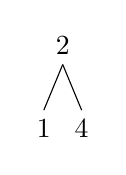
\begin{tikzpicture}
\Tree [.2 1 4 ]
\end{tikzpicture}
\caption{Tree is balanced, no rotation required}
\end{figure}

\begin{figure}[ht]
\centering
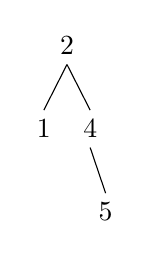
\begin{tikzpicture}
\Tree [.2 1 [.4 \edge[draw=none]; {} 5 ] ]
\end{tikzpicture}
\caption{Tree is balanced, no rotation required}
\end{figure}

\begin{figure}[ht]
\centering
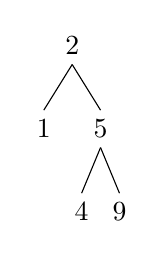
\begin{tikzpicture}
\Tree [.2 1 [.5 4 9 ] ]
\end{tikzpicture}
\caption{Rotated 4 to the left (single)}
\end{figure}

\begin{figure}[ht]
\centering
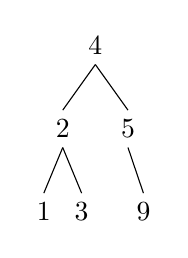
\begin{tikzpicture}
\Tree [.4 [.2 1 3 ] [.5 \edge[draw=none]; {} 9 ] ]
\end{tikzpicture}
\caption{Rotated 2 to the left (double)}
\end{figure}

\begin{figure}[ht]
\centering
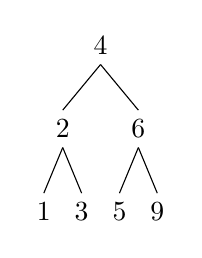
\begin{tikzpicture}
\Tree [.4 [.2 1 3 ] [.6 5 9 ] ]
\end{tikzpicture}
\caption{Rotated 5 to the left (single)}
\end{figure}

\begin{figure}[ht]
\centering
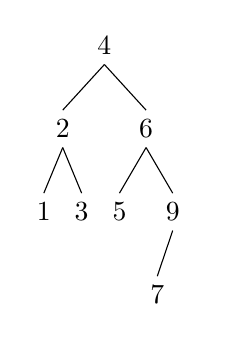
\begin{tikzpicture}
\Tree [.4 [.2 1 3 ] [.6 5 [.9 7 \edge[draw=none]; {} ] ] ]
\end{tikzpicture}
\caption{Tree is balanced, no rotation required}
\end{figure}

\subsection{}


\end{document}